\documentclass[11pt,a4paper]{article}
\usepackage[utf8]{inputenc}
\usepackage{amsfonts}
\usepackage{amssymb}
\usepackage{mdframed}
\usepackage{tikz}
\usetikzlibrary{calc}
\usepackage{tkz-tab}
\usepackage{pgfplots}
\usepackage{xcolor}
\usepackage{fancyhdr}
\usepackage{lastpage}
\usepackage[fleqn]{amsmath}
\setlength{\mathindent}{0pt}

\newcommand{\pdt}{\mathbin{\vcenter{\hbox{\scalebox{0.6}{\textbullet}}}}}

% Spécifications du document
\newcommand{\doctitre}{Géométrie repérée} % Ex: Le second degré
\newcommand{\docniveau}{$1^{\text{re}}$ Spécialité mathématiques} % Ex: $1^{\text{re}}$ Spécialité mathématiques
\newcommand{\doctheme}{Géométrie} %Ex: Algèbre
\newcommand{\doctype}{Cours} % Ex: Démonstrations
\newcommand{\docshorttype}{Cours} % Démo

% Couleurs pour les graphiques
\definecolor{dark_green}{HTML}{008000}

% Paramètres du document
\RequirePackage{geometry}
\geometry{tmargin=1cm,bmargin=1.9cm,lmargin=1.9cm,rmargin=1.9cm}
\renewcommand{\familydefault}{\sfdefault}
\setlength{\parindent}{0pt}
\title{\doctitre}
\author{\docniveau \\ \doctheme\text{ - }\doctype}
\date{}
\fancypagestyle{custom}{
  \fancyhf{}
  \renewcommand{\headrulewidth}{0pt}
  \lfoot{\doctheme\text{ - }\docshorttype}
  \cfoot{\doctitre} % Change \titre to \doctitre
  \rfoot{\thepage/\pageref{LastPage}}
}

% Styles pour les mdframed
\mdfdefinestyle{definitionStyle}{
    leftline=true,
    rightline=false,
    topline=false,
    bottomline=false,
    linewidth=2pt,
    linecolor=black,
    innertopmargin=0pt,
    innerbottommargin=0pt,
    innerrightmargin=0pt,
    innerleftmargin=5pt,
}

\mdfdefinestyle{proprieteStyle}{
    linewidth=1pt,
    linecolor=black,
    innertopmargin=5pt,
    innerbottommargin=5pt,
    innerrightmargin=5pt,
    innerleftmargin=5pt,
}
% ----- DEBUT DU DOCUMENT -----
\begin{document}

% Style et numérotation
\maketitle
\pagestyle{custom}
\thispagestyle{custom}

\section*{I. Équation cartésienne d'une droite et vecteur normal}

\begin{mdframed}[style=definitionStyle]
  \textbf{Définition :} ~\\
  Soit $d$ une droite de vecteur directeur $\vec{u}$. \\
  Un vecteur normal à la droite $(d)$ est un vecteur non nul orthogonal au vecteur $\vec{u}$.
\end{mdframed}

\textbf{Schéma :} ~\\

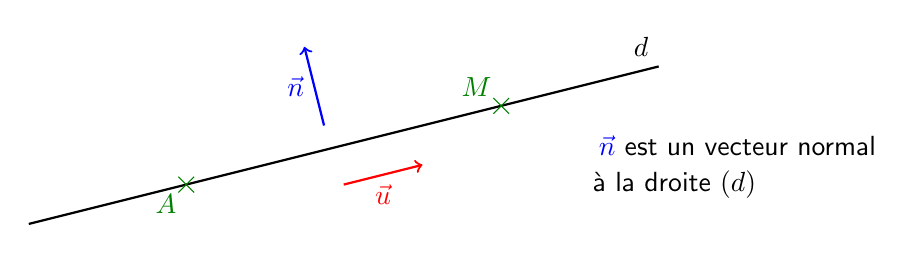
\begin{tikzpicture}
  % Points
  \coordinate (A) at (2,0.5);
  \coordinate (M) at (6,6/4);

  % Droite (d)
  \draw[thick] (0,0) -- (8,2) node[pos=1, above left] {$d$};

  % Points marked with cross
  \draw[dark_green] (A) ++(-0.1,-0.1) -- ++(0.2,0.2);
  \draw[dark_green] (A) ++(-0.1,0.1) -- ++(0.2,-0.2);
  \node[dark_green, below left] at (A) {$A$};

  \draw[dark_green] (M) ++(-0.1,-0.1) -- ++(0.2,0.2);
  \draw[dark_green] (M) ++(-0.1,0.1) -- ++(0.2,-0.2);
  \node[dark_green, above left] at (M) {$M$};

  % Vecteur u et n
  \draw[thick, red, ->] (4,0.5) -- (5,0.75) node[midway, below] {$\vec{u}$};
  \draw[thick, blue, ->] (3.75,1.25) -- (3.5,2.25) node[midway, left] {$\vec{n}$};

  % Texte
  \node at (9,1) {$\color{blue}\vec{n}$ est un vecteur normal};
  \node at (8.20,0.5) {à la droite $(d)$};
\end{tikzpicture}

\text{ }

\begin{mdframed}[style=proprieteStyle]
  \textbf{Propriété :} ~\\
  Soit $a$, $b$ et $c$ trois réels tels que $a$ et $b$ ne sont pas simultanément nuls. \\
  Dans un repère orthonormé, le vecteur $\displaystyle \vec{n}\binom{a}{b}$ est normal à la droite $(d)$ si et seulement si la droite
  admet une équation cartésienne de la forme $ax+by+c=0$ avec $c$ un réel à déterminer.
\end{mdframed}

\textbf{Exemple :} ~\\
On cherche à déterminer une équation cartésienne de la droite $(d)$ passant par le point $A(5;-1)$ et de vecteur normal $\displaystyle \vec{n} \binom{2}{-3}$.
\begin{equation*}
  \begin{split}
    M(x;y)\in (d) & \Leftrightarrow \overrightarrow{AM} \binom{x-5}{y+1} \text{ et } \vec{n} \binom{2}{-3} \text{ sont orthogonaux}\\
    & \Leftrightarrow \overrightarrow{AM}\pdt\vec{n} = 0 \\
    & \Leftrightarrow 2(x-5)-3(y+1)=0 \\
    & \Leftrightarrow 2x-10-3y-3=0 \\
    & \Leftrightarrow 2x-3y-13=0
  \end{split}
\end{equation*}
Donc une équation cartésienne de $(d)$ est $2x-3y-13=0$.

\newpage

\section*{II. Équation cartésienne d'un cercle}

\begin{mdframed}[style=definitionStyle]
  \textbf{Définition :} ~\\
  On appelle cercle de centre $\Omega$ et de rayon $r>0$ l'ensemble des points $M$ du plan qui vérifie $\Omega M=r$.
\end{mdframed}

\begin{mdframed}[style=proprieteStyle]
  \textbf{Propriété de l'équation d'un cercle connaissant son centre et son rayon :} ~\\
  Le plan est muni d'un repère orthonormé $(O,I,J)$. \\
  Soit $C$ le cercle de centre $\Omega(x_0;y_0)$ et de rayon $R$. \\
  Une équation du cercle $C$ est $(x-x_0)^2+(y-y_0)^2=R^2$.
\end{mdframed}

\textbf{Exemple :} ~\\

\begin{minipage}{0.3\textwidth}
  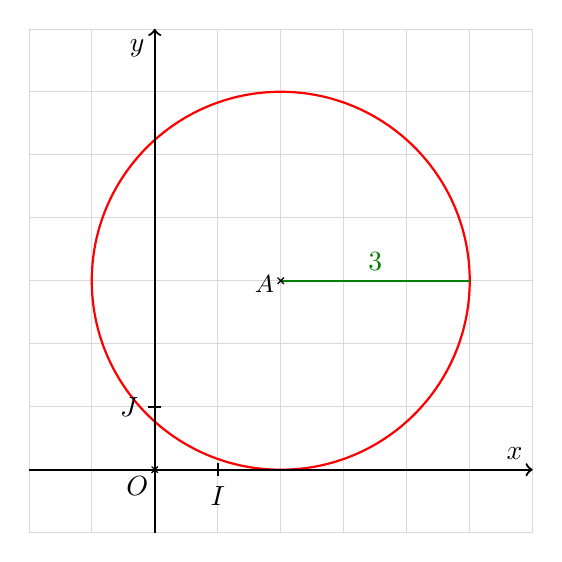
\begin{tikzpicture}[scale=0.8]
    \draw[help lines, gray!30, step=1] (-2,-1) grid (6,7);
    \draw[thick, color=red] (2,3) circle [radius=3];
    \draw[thick,->] (-2,0) -- (6,0) node[above left] {$x$};
    \draw[thick,->] (0,-1) -- (0,7) node[below left] {$y$};
    \draw[thick] (1,0.1) -- (1,-0.1) node[below] {$I$};
    \draw[thick] (0.1,1) -- (-0.1,1) node[left] {$J$};
    \draw[dark_green,thick] (2,3) -- (5,3) node[midway, above] {$3$};
    \draw[thin] (-0.05,-0.05) -- (0.05,0.05) node[below left] {$O$};
    \draw[thin] (-0.05,0.05) -- (0.05,-0.05);
    \coordinate (A) at (2,3);
    \draw[ultra thin, line width=0.4pt] (A) ++(-0.05,-0.05) -- ++(0.1,0.1) (A) ++(-0.05,0.05) -- ++(0.1,-0.1) node[anchor=east] {\small$A$};
  \end{tikzpicture}
\end{minipage}
\hfill
\begin{minipage}{0.6\textwidth}
  On cherche à déterminer l'équation du cercle de centre $A(2;3)$ et de rayon $3$.
  \begin{equation*}
    \begin{split}
      M(x;y)\in C&\Leftrightarrow AM = 3 \\
      & \Leftrightarrow AM^2=9 \text{ avec } AM=\sqrt{(x-2)^2+(y-3)^2} \\
      & \Leftrightarrow (x-2)^2+(y-3)^2=9 \\
      & \Leftrightarrow x^2-4x+4+y^2-6x+9=9 \\
      & \Leftrightarrow x^2+y^2-4x-6x+4=0 \\
    \end{split}
  \end{equation*}
  Une équation cartésienne du cercle de centre $A(2;3)$ et de rayon $3$ est $(x-2)^2+(y-3)^2=9$ ou $x^2+y^2-4x-6x+4=0$. ~\\ ~\\
\end{minipage}

\text{ } \\


\begin{minipage}{0.8\textwidth}
  \begin{mdframed}[style=proprieteStyle]
    \textbf{Propriété de l'équation d'un cercle connaissant son diamètre :} ~\\
    Soit $C$ le cercle de diamètre $[AB]$. \\
    Un point $M(x;y)$ appartient au cercle $C$ si et seulement si $\overrightarrow{MA}\pdt\overrightarrow{MB}=0$.
    Une équation cartésienne du cercle $C$ est donc $(x-x_A)(x-x_B)+(y-y_A)(y-y_B)=0$.
  \end{mdframed}
\end{minipage}
\hfill
\begin{minipage}{0.17\textwidth}
  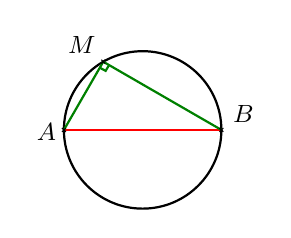
\begin{tikzpicture}[scale=0.5,>=stealth]

    % Définir les coordonnées des points A et B
    \coordinate (A) at (0,0);
    \coordinate (B) at (4,0);

    % Calculer le milieu du segment AB et le rayon du cercle
    \coordinate (M) at ($(A)!0.5!(B)$);
    \pgfmathsetmacro{\radius}{0.485*sqrt(17)}

    % Dessiner un arc de cercle pour représenter le lieu des points possibles pour le point C
    \draw[black, thick] (M) circle (\radius);

    % Choisir un angle pour positionner C sur l'arc de cercle
    \pgfmathsetmacro{\angle}{120}
    \coordinate (C) at ($(M)+(\angle:\radius)$);

    % Dessinez les vecteurs AB et AC
    \draw[red, thick] (A) -- (B) node[midway,anchor=north east] {};
    \draw[dark_green, thick] (A) -- (C) node[midway,anchor=south east] {};
    \draw[dark_green, thick] (C) -- (B) node[midway,anchor=south west] {};

    % % Ajouter une marque d'angle droit en M
    \draw[dark_green, thick] (0.92, 1.575) -- (1.06, 1.5) -- (1.15, 1.65);

    % Marquer les points A, B et M avec des croix plus petites et plus épaisses
    \draw[ultra thin, line width=0.4pt] (A) ++(-0.05,-0.05) -- ++(0.1,0.1) (A) ++(-0.05,0.05) -- ++(0.1,-0.1) node[anchor=east] {\small$A$};
    \draw[ultra thin, line width=0.4pt] (B) ++(-0.05,-0.05) -- ++(0.1,0.1) (B) ++(-0.05,0.05) -- ++(0.1,-0.1) node[anchor=south west] {\small$B$};
    \draw[ultra thin, line width=0.4pt] (C) ++(-0.05,-0.05) -- ++(0.1,0.1) (C) ++(-0.05,0.05) -- ++(0.1,-0.1) node[anchor=south east] {\small$M$};
  \end{tikzpicture}
\end{minipage}

\section*{III. Équation cartésienne d'une parabole}

\begin{mdframed}[style=definitionStyle]
  \textbf{Définition :} ~\\
  Soit $a$, $b$ et $c$ trois réels tels que $a\not=0$. \\
  Soit $f$ une fonction polynôme du second degré définie par $f(x)=ax^2+bx+c$. \\
  La courbe représentative de la fonction $f$ qui a pour équation $y=ax^2+bx+c$ est une parabole.
\end{mdframed}

\begin{mdframed}[style=proprieteStyle]
  \textbf{Propriété :} ~\\
  Cette courbe représentative admet pour axe de symétrie de la droite d'équation $\displaystyle x=\frac{-b}{2a}$ et pour sommet le point $\displaystyle S\left(\frac{-b}{2a};f\left(\frac{-b}{2a}\right)\right)$.
\end{mdframed}

\textbf{Exemple :} ~\\
On cherche à déterminer le sommet et l'axe de symétrie de la parabole d'équation $y=-x^2+2x-5$. \\

\begin{minipage}{0.5\textwidth}
  Axe de symétrie : \\
  On a $a=-1$, $b=2$ et $c=-5$. \\
  On calcule $\displaystyle x=\frac{-b}{2a}=\frac{-2}{2(-1)}=1$. \\
  Donc l'axe de symétrie de la parabole est $x=1$. \\
\end{minipage}
\hfill
\begin{minipage}{0.5\textwidth}
  Sommet : \\
  Donc le sommet a pour abscisse $1$. \\
  Son ordonnée est $y=-1^2+2\times1-5=-4$. \\
  Donc $S\left(1;-4\right)$
  \vspace*{20pt}
\end{minipage}

\end{document}
% ----- FIN DU DOCUMENT -----